%% Ternary complex model
%% FigInline3MonomerTree.tex
%% Unused packages and definitions removed; TikZ/PGFPlots source formatted.

\documentclass{standalone}

\usepackage{tikz}
\usetikzlibrary{arrows}

\def\b{\mathsf{b}}
\def\c{\mathsf{c}}
\def\d{\mathsf{d}}
\def\x{\mathsf{x}}

\def\kappab{\kappa_{\b}}
\def\kappac{\kappa_{\c}}
\def\kappad{\kappa_{\d}}
\def\kappax{\kappa_{\x}}

\def\etabc{\eta_{\b\c}}
\def\etacd{\eta_{\c\d}}

\def\etabc{\eta_{\b\c}}
\def\etacd{\eta_{\c\d}}

\begin{document}

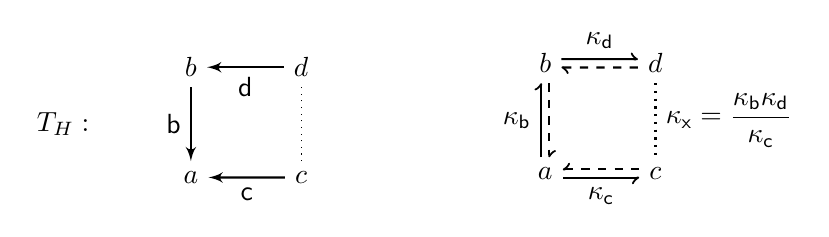
\begin{tikzpicture}[scale=0.9,style=thick,shorten >=0pt,shorten <=0pt,>=latex']

    \begin{scope}[node distance=1.4cm]
        \draw (0,0) node (B) {$b$};
        \node[below of=B] (A) {$a$};
        \draw[->,thick] (B) to node[left,align=center] (BB) {$\b$} (A);
        \node[right of=A] (C) {$c$};
        \draw[<-,thick] (A) to node[below] {$\c$} (C);
        \node[right of=B] (D) {$d$};
        \draw[->,thick] (D) to node[below] {$\d$} (B);
        \draw[dotted,thin] (C) to (D);
        \node[left of=BB] {$T_H:$};
    \end{scope}

    \begin{scope}[node distance=1.4cm,xshift=5cm,yshift=-1.5cm]
        \draw (0,0) node (AAP) {$a$};
        \node[above of=AAP] (ABP) {$b$};

        \node[right of=AAP] (BAP) {$c$};
        \node[right of=ABP] (BBP) {$d$};
        \node[right of=ABP] (X) {};

        \draw[-left to,thick,transform canvas={xshift=-1.5pt}] (AAP) to node[left] {$\kappa_\b $} (ABP);
        \draw[dashed,-left to,thick,transform canvas={xshift=1.5pt}] (ABP) to (AAP);

        \draw[dotted] (BBP) to node[right] {$\kappax = \displaystyle \frac{\kappab\kappad}{\kappac}$} (BAP);

        \draw[dashed,right to-,thick,transform canvas={yshift=1.5pt}] (AAP) to (BAP);
        \draw[right to-,thick,transform canvas={yshift=-1.5pt}] (BAP) to  node[below] {$\kappa_\c$} (AAP);

        \draw[-left to,thick,transform canvas={yshift=1.5pt}] (ABP) to node[above] {$\kappa_\d $} (BBP);
        \draw[dashed,-left to,thick,transform canvas={yshift=-1.5pt}] (BBP)to (ABP);
    \end{scope}

\end{tikzpicture}

\end{document}

